\section{A Model of Unrecognized Statehood} 
We model a dispute over a piece of territory that is controlled by a secessionist group and also claimed by a home state. Because our model incorporates the incentives and actions of international actors, it is about to both articulate the mechanisms that create these persistent stalemates and to assess the consequences, intended and otherwise, of outside actors' attempts to foster their desired outcome.

\subsection{The Players}

We construct a model with four players: the secessionist elite ($s$), which seeks recognized independence; the central government of the home state ($g$) from which $s$ is attempting to secede, which seeks reunification; and two outside actors:the patron ($p$) and the international community ($c$).

Player $c$ prefers reunification to recognized independence---a preference that is common to most states, and especially among those that fear the prospect of secessionist movements within their own borders. In practice we often observe groups of states like the OECD or the UN acting in this capacity. We also assume player $c$ prefers peace to war; this implies that player $c$ will not fund a military buildup that it expects will induce war.

In contrast, Player $p$ most prefers recognized independence and opposed independence, aligning its interests with the secessionists. We refer to $p$ as the patron because $p$ contributes resources to the unrecognized state in the status quo equilibrium. Patrons choose to contribute resources to secessionists for one or more of several reasons: 1) As an efficient mechanism for imposing costs on the home state (Salehyan et al., 2012), e.g. as Russia does to Georgia via South Ossetia and Abkhazia; 2) ethnic solidarity with the secessionists (e.g. Turkey's support of the Turkish Republic of Northern Cyprus); 3) hope of eventual annexation of the disputed territory (e.g. Armenia's support of Nagorno-Karabakh). Although there may exist patrons whose most-preferred outcome is the status quo, we examine the case where the patron's most preferred outcome is independence because this is the condition under which the status quo is least likely. We will show that even in this circumstance the status quo remains an equilibrium outcome.

We do not restrict the preferences and capabilities for players $g$ and $s$, with one exception. We assert that the payoffs for the party that cedes the issue of status (independence vs. reunification) are consistently low. This reflects the fact that the issue of status is indivisible and highly valued by each side and that many of the payments that could be offered are not credible (Licklider, 1995; Walter 1997, 2002; Doyle and Sambanis, 2006; Fearon and Laitin, 2007; Schultz, 2010).


\subsection{Details of the Dynamic Game}
\label{sec:structure}

The game begins at a status quo in which the secessionist elite controls at least some of the disputed territory but cannot gain international recognition unless the central government cedes its claim to the territory. This condition is archetypical of cases in which a militarily successful war of secession ends in a ceasefire.  

There are an infinite number of discrete periods $t=1,2,\ldots$. Play proceeds in each period $t$ as follows (and as shown in Figure 1) until an absorbing state is reached.

\begin{figure}
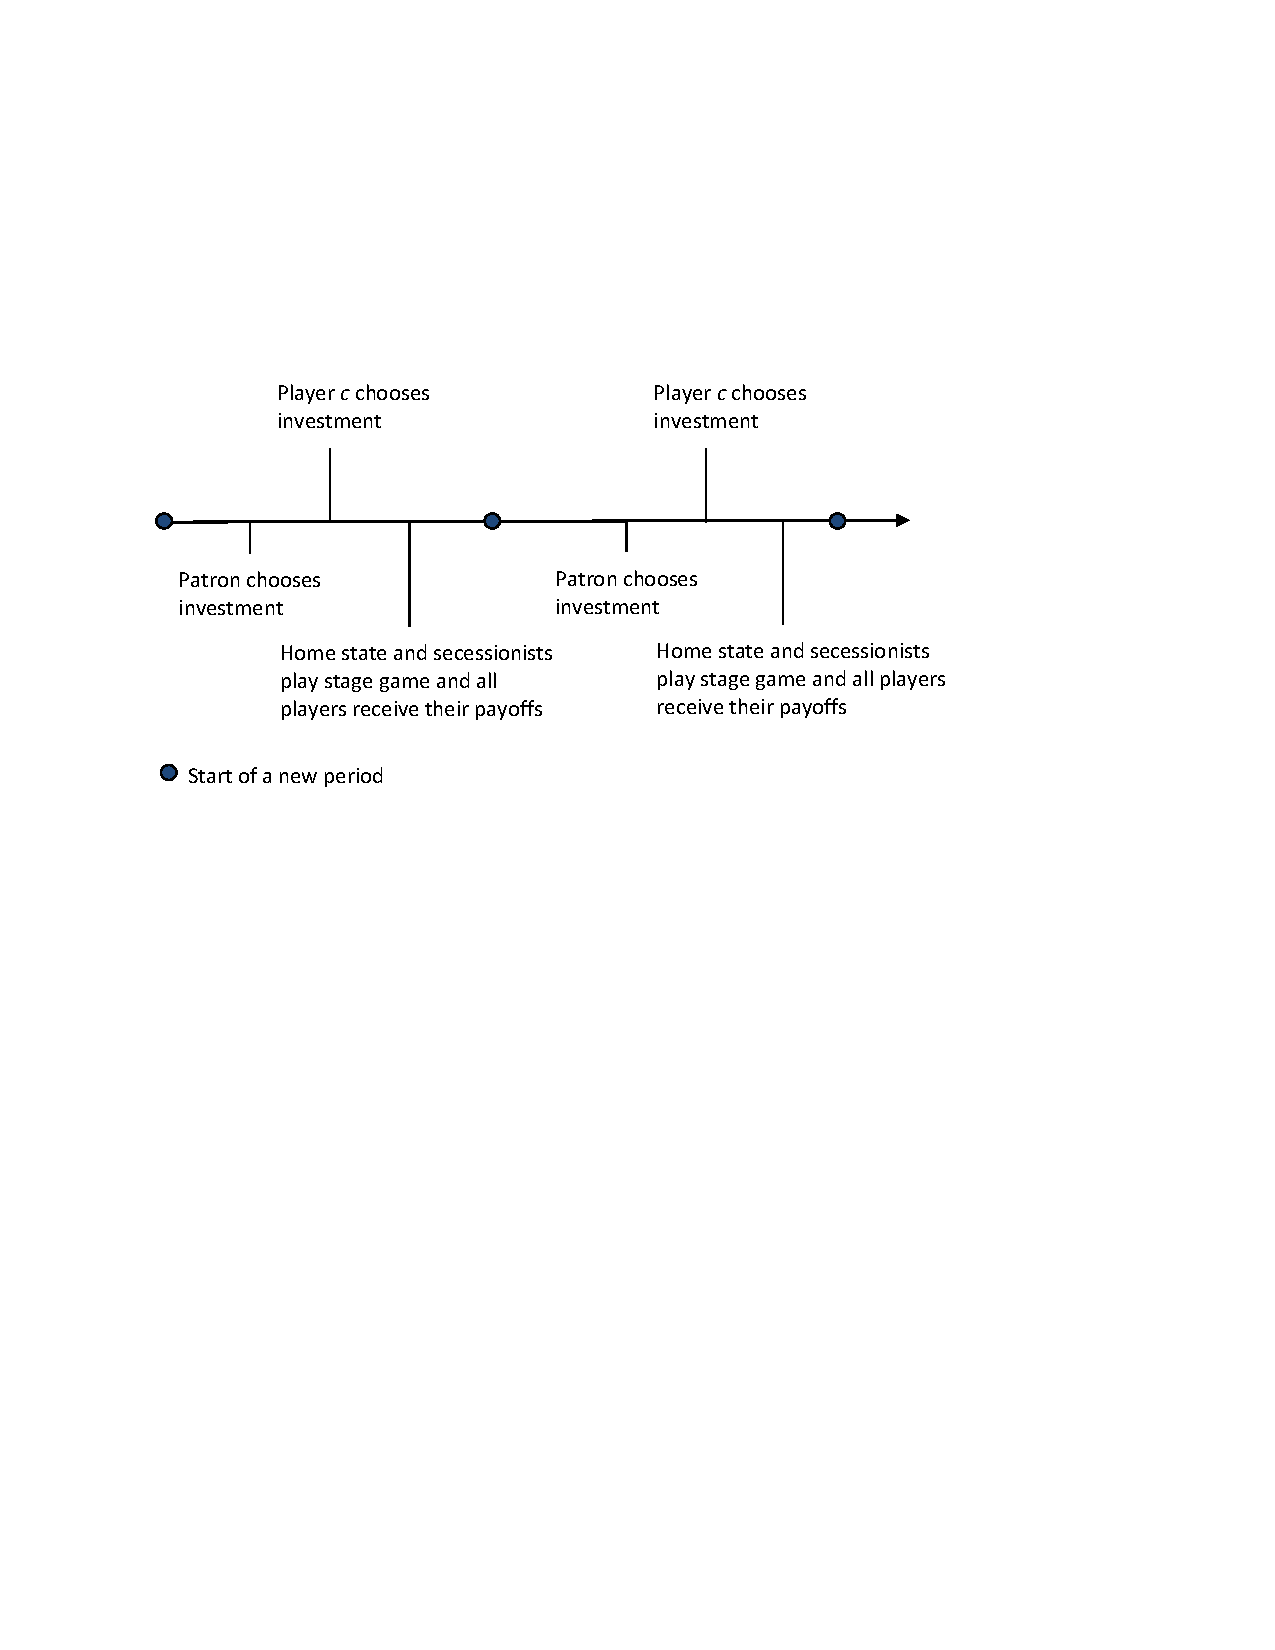
\includegraphics{Timeline2.pdf}
\caption{Timeline}
\end{figure}

\begin{enumerate} 
\item $p$ chooses an investment level to influence the payoffs of $s$ and $g$. 
 
\item $c$ chooses an investment level to influence the payoffs of $s$ and $g$.
 
\item Conflict Stage Game: $s$ and $g$ play a stage game in which each chooses simultaneously from the following actions: Fight, Status Quo, Cede. 
\end{enumerate}

The payoffs at the end of a period are determined by these actions and the values of state variables that keep track of the value of the status quo, losing and winning the issue of status for the secessionists and government respectively. 

All the state variables except for the secessionists' status quo payoffs remain unchanged from period to period unless players $p$ or $c$ make an investment. The status quo payoffs for the secessionists are automatically reduced by $\mu$ each period. The steady reduction by $\mu$ represents the costs of non-recognition.

Only two outcomes of the stage game do not lead to absorbing states. If both $s$ and $g$ play Status Quo, then the status quo persists. Likewise, if both states simultaneously play Cede, we assume that both renege immediately and that the status quo is preserved for that period. In this case neither player has demonstrated a willingness to give up more than the other.

If either $s$ or $g$ plays Cede while the other plays Fight or Status Quo, the game ends with payoffs in every subsequent period given by the corresponding payoffs in the stage game. Therefore, if one player agrees to cede while the other player chooses to remain in the status quo or fight, the result is a negotiated settlement benefiting the player who did not cede. 

There are three ways to end up in war: either of the parties may attack first, or both may attack simultaneously. We use a lottery to determine whether the secessionists or government wins the war. Victory would, among other things, allow an unrecognized state to force recognition by the home state government.

Future payoffs are discounted with a common parameter $\de \in [0,1]$. Therefore payoffs for the entire game for player $i\in \{s, g, p, c\} $ can be expressed by the discounted stream of payments $\Sigma_{t=1}^{\infty} \de^{t-1} U_i^t $ where $U_i^t$ is player $i$'s payoff in period $t$.

The payoff functions and all parameters, including probabilities in the war lottery, are common knowledge for all players.




\section{Explaining Outcomes of Secessionist Conflicts: The ``Status Quo'' Equilibrium} 
\label{sec:main}

Despite the preferences of the international community for peace, the most common outcome of secessionist conflicts in the post-WWII period has been reunification with the home state via outright military reconquest. By contrast, reunification through negotiated settlement has been very rare. In this section, we use a game theoretic model to explain the outcome that we find the most puzzling: perpetual unrecognized statehood.

Unrecognized states are frequently viewed as temporary phenomena or as non-equilibrium outcomes attributable to players' misperceptions of the strategic situation, or their fundamental irrationality. Our central result shows that unrecognized statehood can be an equilibrium outcome capable of being sustained in perpetuity by fully rational, perfectly informed actors. 

We begin by listing a set of restrictions on the preferences of the actors and their resources for which we can guarantee that unrecognized statehood is an equilibrium outcome.

\begin{definition}
\emph{The class $\mathcal{G}$ includes all those games for which following restrictions are satisfied:}

\begin{enumerate}
\item \textit{For both players $g$ and $s$, remaining in the status quo is better than ceding at the beginning of the game.}\label{res:1}

\item \textit{For both players $g$ and $s$, the expected outcome under war is worse than the status quo at the beginning of the game.}\label{res:2}

\item \textit{Either the secessionists prefer ceding to war or the patron's disutility from war is greater than the per-period cost of offsetting the deterioration in the secessionists' status quo payoffs.}\label{res:new}

\item \textit{Reunification is more important for the patron to avoid than for the international community to achieve.}\label{res:3}

\item  \textit{Recognition of the secessionist state is more important for the international community to avoid than for the patron to achieve.}\label{res:4}

\item  \textit{The patron can afford to deter player $c$ from inducing reunification at the beginning of the game.}\label{res:5}

\item \textit{The patron can afford to pay to maintain the status quo.}\label{res:6}

\end{enumerate}
\end{definition}

We can show that at least one status quo equilibrium exists for any game satisfying the restrictions in Definition 1. Our concept of equilibrium is stationary Markov equilibrium in which strategies ignore all details of the history aside from the current state.

The state is a vector of six variables comprised of the payoffs from the status quo, ceding, and winning the issue of status for each of the two inside actors. Player $c$ dislikes war and so will never invest in either state variable associated with winning since they increase the likelihood that one of the inside actors chooses to fight. It would also not invest in the government's payoffs from ceding. The patron will never invest in the government's payoffs from winning or the secessionists' payoffs from ceding, and it will not invest in the government's status quo payoffs because player $c$ will not invest in the government's payoffs from war so there is no need to counter such an investment. This leaves three state variables in which each outside actor might invest, which we address while defining the Status Quo Equilibrium. 

\begin{definition}
A Status Quo Equilibrium is a stationary Markov equilibrium in which the outcome is perpetual unrecognized statehood.

The strategies for the government and secessionists in this equilibrium are to play their best responses given the continuation values induced by the investments of the outside actors. Unless otherwise noted below, playing Status Quo is the best response for both inside actors in terms of continuation values.

The strategies for the outside actors in period $t$ are:

\begin{enumerate}
	\item The patron invests enough in the secessionists Status Quo payoffs to deter Player $c$ from investing in the secessionists' payoffs from Ceding. Otherwise, Player $c$ invests enough to induce the secessionists to play Cede.

	\item Player $c$ is prepared to counter the largest investment the patron is willing to make in the government's payoffs from ceding by making a counter-investment in the government's status quo payoffs. If the patron were to make an investment larger than its willingness to pay, Player $c$ would not counter and the government would play Cede.
	
	\item Investments by player $c$ in the secessionists' status quo payoffs deter the patron from investing in the secessionists' payoffs from winning the conflict via fighting. If the patron were to make an investment larger than its willingness to pay, Player $c$ would not counter and the secessionists would play Fight.
\end{enumerate}
\end{definition}

To understand the construction of this equilibrium, notice that there are three possible ways to disrupt the Status Quo: (1) the international community can provoke the secessionists to Cede, (2) the patron can provoke the government to cede, or (3) the patron can provoke the secessionists to fight.\footnote{The international community might also provoke the government to fight, but it is assumed to avoid conflict.} In order to establish that the Status Quo Equilibrium exists, it must be shown that each of these three deviations will be deterred.

Since the patron moves first, the only investment that takes place in the Status Quo Equilibrium is the patron's investment in the status quo payoffs of the secessionists to deter the international community from provoking the secessionists to cede the issue of sovereignty. This requires that Restrictions (\ref{res:new}) and (\ref{res:3}) of Definition 1 hold. The patron must also have sufficient resources as per Restrictions (\ref{res:5}) and (\ref{res:6}).

The international community's willingness to counteract investments by the patron toward the other two disturbances (i.e., Restriction (\ref{res:4})) implies that there will be no investments in equilibrium in cases (2) and (3). Case (3) also requires Restrictions (\ref{res:3}) of Definition 1 and the implicit assumption that the patron is not able to skew the odds of the secessionists winning the conflict in a way that cannot be nullified by the international community. 

If, however, off-path investments are ever made such that Status Quo does not yield the highest continuation value for one of the players, that player will play Cede or Fight and the game will end.

Equilibrium actions are for the patron to maintain the status quo by investing enough to overcome the deterioration in the secessionists' status quo payoffs; for the international community to not invest and for both inside actors to play Status Quo each period.

\begin{proposition}
	For any game in the class of games $\mathcal{G}$, there exists at least one Status Quo Equilibrium.
\end{proposition}

The full proof of Proposition 1 is available in Buzard, Graham and Horne (2017).


\subsection{Discussion}

The existence and durability of this not-infrequently observed status quo equilibrium is counterintuitive on two levels. First, the large, relatively rich international community is outspent by a relatively small, less-resourced patron; second, unrecognized statehood is a stable equilibrium in spite of being undesirable to all players. The key condition leading to this outcome is that each outside actor's willingness to pay to achieve its most preferred outcome is outweighed by the other's desire to avoid it's least desired outcome. An ongoing unresolved conflict results.

Despite its high costs, this equilibrium is quite robust. Because player $c$ and the patron can adjust contributions to reflect changing conditions on the ground, exogenous shocks that might otherwise have the potential to alter the equilibrium have their strategic impact nullified. For example, while a drought in the unrecognized state might decrease the secessionist elite's payoffs from the status quo and increase their need for international trade and assistance, additional humanitarian and economic assistance from the patron can offset the effects of the shock and preserve the status quo.

\subsection{Alternative Outcomes}
\label{sec:alt}

First, note that the restrictions in Definition 1 are sufficient but not necessary. For example, if the status quo initially has a much higher long term payoff than the next best alternative for the secessionists, Restriction (\ref{res:6}) need not be met to maintain the status quo in the short run. The inequality \emph{will} bind for some set of periods $t \geq 1$ because the secessionist payoffs from the status quo decrease over time. 

On the other hand, the restrictions in Definition 1 also \emph{do not} provide for a unique equilibrium, or even a unique equilibrium outcome. In fact, at least one additional equilibrium outcome always coexists with the status quo outcome. The equilibria may involve (Fight,Fight), (Fight,Cede) and/or (Cede,Fight) as outcomes of the stage game.

There are at least two takeaways from the multiplicity of equilibrium outcomes. First, it indicates that there may be an important role for external actors to play in coordinating expectations about which equilibrium will be played, and in the absence of such coordination, equilibrium switching from the status quo equilibrium to one of the other outcomes is possible. Second, most of the types of outcomes that we observe in the post-WWII era are consistent with the set of restrictions outlined in Proposition 1 that support the status quo outcome. 

\section{The Impact of Economic Sanctions}
\label{sec:sanctions}

In Section~\ref{sec:main}, we considered the outside actors' abilities to make investments to increase the various payoffs of the home state government and the secessionists. Player $c$, in particular, often employs another option by joining the home state in enforcing economic sanctions against the unrecognized state, an action that \emph{reduces} the secessionists' payoffs from the status quo. Note that this may be particularly effective if $c$ is a large coalition of states acting in concert. 

Let us begin with the simplest case, in which the sanctions affect only the secessionists' status quo payoffs, as when the imposition of sanctions has a negative impact on the economy of the unrecognized state. In this case, the effect of sanctions on the unrecognized state's choice is ambiguous. 

\begin{proposition}
Assume the restrictions of \emph{Definition 1} hold in the absence of sanctions and that sanctions affect only player $s$'s payoffs to maintaining the Status Quo.  In order for sanctions to lead to ceding by the secessionists, the following are required:

\begin{enumerate}
\item \textit{The patron must either be unable or find that it is not worthwhile to invest the additional amount now required to maintain the status quo.}

\item \textit{The patron must either be unable or find that it is not worthwhile to invest to instigate fighting by the secessionists.}

\item \textit{The secessionists' continuation value from playing Cede must be higher than their continuation value from playing Fight.}
\end{enumerate}

\end{proposition}

The proof of Proposition 2 can be found in Buzard, Graham and Horne (2017).

If Condition 1 fails, player $p$ will continue to invest to prevent reunification as in Proposition 1. If Conditions 2 or 3 fail, sanctions will lead to fighting initiated by the secessionists---either supported by the patron, or without its support in the case of Condition 3. Note here from Condition 2 that sanctions can induce investment behavior by the patron that was ruled out under the restrictions of Definition 1: the goal of sanctions is to destabilize the Status Quo Equilibrium and they certainly can achieve that goal but there may be unintended consequences, most notably the initiation of war by the secessionists. 

We can add realism by allowing sanctions to have a negative effect not only on the economy (the status quo payoffs) but also on the military capabilities of the secessionists (the expected payoffs from war). This is an important extension because one motivation for sanctions is often precisely that -- to weaken the military capability of the secessionists. 

In the model, this is represented as reducing the secessionists' probability of victory in the war lottery. This should serve to increase the range of parameters over which the conditions of Proposition 2 hold. However, at the same time, the home government experiences changes of the same magnitude and opposite sign in its war lottery, increasing its payoffs from playing Fight. 

\begin{proposition}
Assume the restrictions of \emph{Definition 1} hold in the absence of sanctions and that sanctions affect both player $s$'s status quo payoffs and its military capabilities. The parameter space over which a war will be initiated by the home state is increasing in the magnitude of the sanctions' impact on the secessionists' military capabilities.
\end{proposition}

It is immediate that the stronger is the impact of sanctions on the secessionists military, the stronger is the effect on the home government's value of fighting and the greater is the range of parameters over which this change in payoffs will lead to a change in behavior.

Thus, Propositions 2 and 3 imply that sanctions are both wealth destroying and violence increasing. The sanctions destroy wealth directly by damaging the economy of the secessionist region and lowering the secessionists' payoffs from the status quo. If the degradation of status quo payoffs are not offset by the patron and if the secessionists' continuation value from fighting exceeds that from the status quo before the continuation value from ceding does, the secessionists will initiate war. Conversely, if the sanctions degrade the secessionists military capabilities sufficiently, it induces the home state to fight.


